\documentclass{article}

\usepackage{tikz}
\usetikzlibrary{automata, positioning}

\begin{document}
\pagestyle{empty}

\def\layersep{1.5cm}

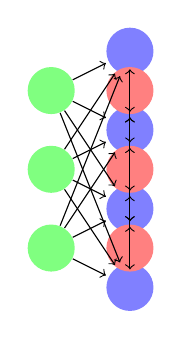
\begin{tikzpicture}[shorten >=1pt,->,draw=black, node distance=\layersep]
    \tikzstyle{every pin edge}=[<-,shorten <=1pt]
    \tikzstyle{neuron}=[circle,fill=black!25,minimum size=17pt,inner sep=0pt]
    \tikzstyle{input neuron}=[neuron, fill=green!50];
    \tikzstyle{output neuron}=[neuron, fill=red!50];
    \tikzstyle{hidden neuron}=[neuron, fill=blue!50];
    \tikzstyle{annot} = [text width=4em, text centered]

    % Draw the input layer nodes
    \foreach \name / \y in {1,...,3}
    % This is the same as writing \foreach \name / \y in {1/1,2/2,3/3,4/4}
        \node[input neuron, 
        %pin=left:Input \#\y
        ] (I-\name) at (0,-\y) {};

    % Draw the hidden layer nodes
    \foreach \name / \y in {1,...,4}
        \path[yshift=0.5cm]
            node[hidden neuron] (H-\name) at (\layersep,-\y cm) {};

    % Draw the output layer node
%    \node[output neuron,
    %pin={[pin edge={->}]right:Output}, 
%    right of=H-3] (O) {};
    \foreach \name / \y in {1,...,3}
        \path[yshift=0.0cm]
            node[output neuron] (O-\name) at (\layersep+\layersep,-\y cm) {};

    % Connect every node in the input layer with every node in the
    % hidden layer.
    \foreach \source in {1,...,3}
        \foreach \dest in {1,...,4}
            \path (I-\source) edge (H-\dest);

    % Connect every node in the hidden layer with the output layer
    \foreach \source in {1,...,4}
    	\foreach \dest in {1,...,3}
	        \path (H-\source) edge (O-\dest);

    % Annotate the layers
   % \node[annot,above of=H-1, node distance=1cm] (hl) {Hidden layer};
    %\node[annot,left of=hl] {Input layer};
    %\node[annot,right of=hl] {Output layer};
\end{tikzpicture}

\newpage

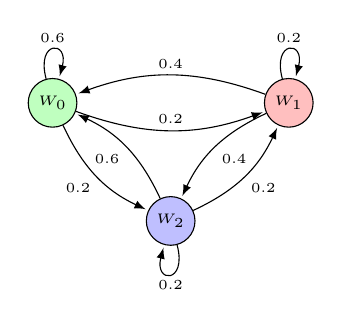
\begin{tikzpicture}
\tiny
        % Draw the states
        \node[state, fill=green!25] at (0, 0)      (a)     {$W_0$};
        \node[state, fill=red!25] at (3, 0)      (b)     {$W_1$};
        \node[state, fill=blue!25] at (1.5, -1.5) (c) {$W_2$};
        % Connect the states with arrows
        \draw[every loop,
              auto=right,
              >=latex]
            (a) edge[bend right=20]            node {0.2} (c)
            (a) edge[bend right=20, auto=left] node {0.2} (b)
            (b) edge[bend right=20]            node {0.4} (a)
            (b) edge[bend right=20, auto=left] node {0.4} (c)
            (c) edge[bend right=20]            node {0.2} (b)
            (c) edge[bend right=20, auto=left] node {0.6} (a)
            (a) edge[loop above]             node {0.6} (a)
            (b) edge[loop above]             node {0.2} (b)
            (c) edge[loop below]             node {0.2} (c);
\end{tikzpicture}
\hspace{15mm}
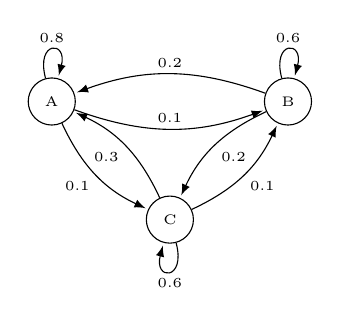
\begin{tikzpicture}
\tiny
        % Draw the states
        \node[state] at (0, 0)      (a)     {A};
        \node[state] at (3, 0)      (b)     {B};
        \node[state] at (1.5, -1.5) (c) {C};
        % Connect the states with arrows
        \draw[every loop,
              auto=right,
              >=latex]
            (a) edge[bend right=20]            node {0.1} (c)
            (a) edge[bend right=20, auto=left] node {0.1} (b)
            (b) edge[bend right=20]            node {0.2} (a)
            (b) edge[bend right=20, auto=left] node {0.2} (c)
            (c) edge[bend right=20]            node {0.1} (b)
            (c) edge[bend right=20, auto=left] node {0.3} (a)
            (a) edge[loop above]             node {0.8} (a)
            (b) edge[loop above]             node {0.6} (b)
            (c) edge[loop below]             node {0.6} (c);
\end{tikzpicture}

\newpage

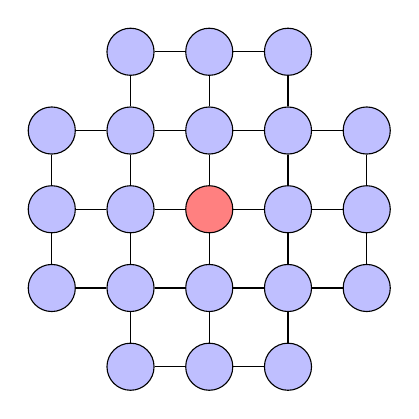
\begin{tikzpicture}
\tiny
        % Draw the states
%        \node[state] at (0, 0)      (1a)     {};
        \node[state, fill=blue!25] at (1, 0)      (1b)     {};
        \node[state, fill=blue!25] at (2, 0)      (1c)     {};
        \node[state, fill=blue!25] at (3, 0)      (1d)     {};
%        \node[state] at (4, 0)      (1e)     {};
        \node[state, fill=blue!25] at (0, -1)     (2a)     {};
        \node[state, fill=blue!25] at (1, -1)     (2b)     {};
        \node[state, fill=blue!25] at (2, -1)     (2c)     {};
        \node[state, fill=blue!25] at (3, -1)     (2d)    {};
        \node[state, fill=blue!25] at (4, -1)     (2e)    {};
        \node[state, fill=blue!25] at (0, -2)     (3a)    {};
        \node[state, fill=blue!25] at (1, -2)     (3b)    {};
        \node[state, fill=red!50] at (2, -2)     (3c)    {};
        \node[state, fill=blue!25] at (3, -2)     (3d)    {};
        \node[state, fill=blue!25] at (4, -2)     (3e)    {};
        \node[state, fill=blue!25] at (0, -3)     (4a)    {};
        \node[state, fill=blue!25] at (1, -3)     (4b)    {};
        \node[state, fill=blue!25] at (2, -3)     (4c)    {};
        \node[state, fill=blue!25] at (3, -3)     (4d)    {};
        \node[state, fill=blue!25] at (4, -3)     (4e)    {};
%        \node[state] at (0, -4)     (5a)    {};
        \node[state, fill=blue!25] at (1, -4)     (5b)    {};
        \node[state, fill=blue!25] at (2, -4)     (5c)    {};
        \node[state, fill=blue!25] at (3, -4)     (5d)    {};
%        \node[state] at (4, -4)     (5e)    {};
%\draw[]  (1a) edge (1b);
\draw[]  (1b) edge (1c);
\draw[]  (1c) edge (1d);
%\draw[]  (1d) edge (1e);
\draw[]  (2a) edge (2b);
\draw[]  (2b) edge (2c);
\draw[]  (2c) edge (2d);
\draw[]  (2d) edge (2e);
\draw[]  (3a) edge (3b);
\draw[]  (3b) edge (3c);
\draw[]  (3c) edge (3d);
\draw[]  (3d) edge (3e);
\draw[]  (4a) edge (4b);
\draw[]  (4b) edge (4c);
\draw[]  (4c) edge (4d);
\draw[]  (4d) edge (4e);
%\draw[]  (3a) edge (3b);
\draw[]  (5b) edge (5c);
\draw[]  (5c) edge (5d);
%\draw[]  (3d) edge (3e);

\draw[]  (2a) edge (3a);
\draw[]  (3a) edge (4a);
\draw[]  (1b) edge (2b);
\draw[]  (2b) edge (3b);
\draw[]  (3b) edge (4b);
\draw[]  (4b) edge (5b);
\draw[]  (1c) edge (2c);
\draw[]  (2c) edge (3c);
\draw[]  (3c) edge (4c);
\draw[]  (4c) edge (5c);
\draw[]  (1d) edge (2d);
\draw[]  (2d) edge (3d);
\draw[]  (3d) edge (4d);
\draw[]  (4d) edge (5d);
\draw[]  (2e) edge (3e);
\draw[]  (3e) edge (4e);

%\draw[]
%(1a) edge[]            node {0.1} (1b);

        % Connect the states with arrows
%        \draw[every loop,
%              auto=right,
%              >=latex]
%            (a) edge[bend right=20]            node {0.1} (c)
%            (a) edge[bend right=20, auto=left] node {0.1} (b)
%            (b) edge[bend right=20]            node {0.2} (a)
%            (b) edge[bend right=20, auto=left] node {0.2} (c)
%            (c) edge[bend right=20]            node {0.1} (b)
%            (c) edge[bend right=20, auto=left] node {0.3} (a)
%            (a) edge[loop above]             node {0.8} (a)
%            (b) edge[loop above]             node {0.6} (b)
%            (c) edge[loop below]             node {0.6} (c);
\end{tikzpicture}

% End of code
\end{document}